\subsection{Временные ряды}

    На временных рядах можно продемонстрировать как различные виды шума влияют на поведение системы.

    На рисунке \ref{time_series_x_0_06_a_1_b_0_56} изображено поведение модели без добавления каких-либо шумов. Видно, что значения переменной \(x\) с течением времени стабилизируются. Численность популяции фактически остается неизменной.

    \begin{figure}
        \centering
        \subfloat[Для модели (\ref{origin})]{
            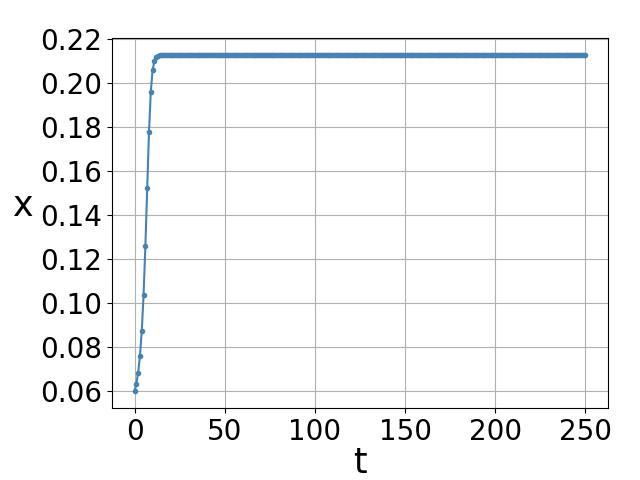
\includegraphics[width=0.5\textwidth]{stochastic/images/time_series_x_0_06_a_1_b_0_56.jpg}
            \label{time_series_x_0_06_a_1_b_0_56}
        }
        \subfloat[Для модели (\ref{alpha_chaos})]{
            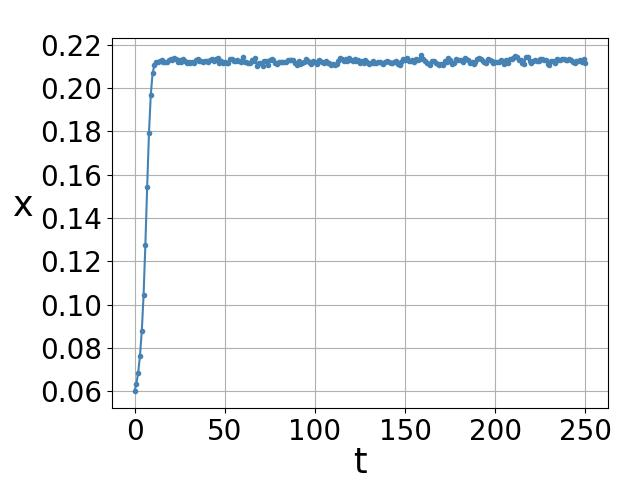
\includegraphics[width=0.5\textwidth]{stochastic/images/time_series_x_0_06_a_1_b_0_56_alpha_chaos_epsilon_0_004.jpg}
            \label{time_series_x_0_06_a_1_b_0_56_alpha_chaos_epsilon_0_004}
        }  

        \subfloat[Для модели (\ref{beta_chaos})]{
            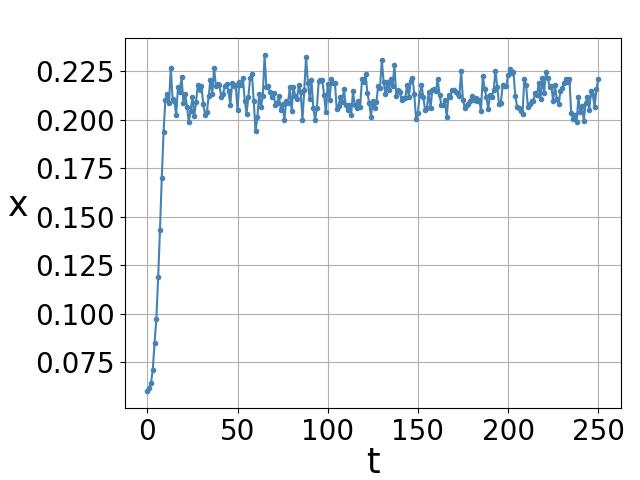
\includegraphics[width=0.5\textwidth]{stochastic/images/time_series_x_0_06_a_1_b_0_56_beta_chaos_epsilon_0_004.jpg}
            \label{time_series_x_0_06_a_1_b_0_56_beta_chaos_epsilon_0_004}
        }
        \subfloat[Для модели (\ref{additive_chaos})]{
            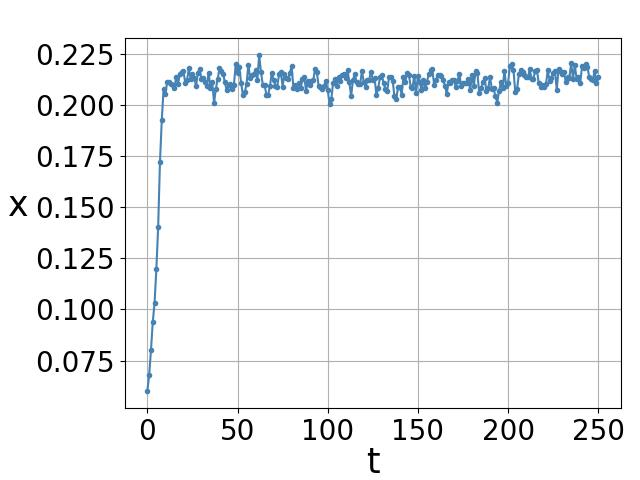
\includegraphics[width=0.5\textwidth]{stochastic/images/time_series_x_0_06_a_1_b_0_56_additive_chaos_epsilon_0_004.jpg}
            \label{time_series_x_0_06_a_1_b_0_56_additive_chaos_epsilon_0_004}
        }
        
        \captionsetup{justification=centering}
        \caption{Временные ряды при \(\alpha = 1, \beta = 0.56, x_0 = 0.06, \varepsilon = 0.004\)}
    \end{figure}

    Далее на рисунках \ref{time_series_x_0_06_a_1_b_0_56_alpha_chaos_epsilon_0_004}, \ref{time_series_x_0_06_a_1_b_0_56_beta_chaos_epsilon_0_004}, \ref{time_series_x_0_06_a_1_b_0_56_additive_chaos_epsilon_0_004} представлены временные ряды для различных видов шума: 

    \begin{enumerate}[a)]
        \setcounter{enumi}{1}
        \item \(\alpha\)-шум
        \item \(\beta\)-шум
        \item аддитивный шум
    \end{enumerate}

    Все варианты рассматриваются с одной и той же интенсивностью шума \(\varepsilon = 0.004\). 
        
    Вид шума влияет на величину разброса значений численности популяции. И если в модели (\ref{origin}) численность популяции стабилизировалась и переставала хоть сколько-нибудь меняться, то в моделях (\ref{alpha_chaos}), (\ref{beta_chaos}) и (\ref{additive_chaos}) численность постоянно колеблется. Эти колебания происходят в рамках некоторого интервала значений. Численность популяции не растет и не уменьшается на какую-то значительную величину. Но такое поведение наблюдается не всегда.

    Для демонстрации другого возможного поведения интенсивность шума была увеличена до \(\varepsilon = 0.04\). На графике \ref{time_series_x_0_06_a_1_b_0_56_beta_chaos_epsilon_0_04_fall} видна ситуация, когда в одном эксперименте из-за шума траектория модели ушла в ноль. В другом эксперименте с точно такими же вводными параметрами траектория не ушла в ноль, т.е. популяция выживала на протяжении анализируемого интервала времени. Данный пример изображен на картинке \ref{time_series_x_0_06_a_1_b_0_56_beta_chaos_epsilon_0_04_alive}. Аналогичные эффекты наблюдаются при других видах шума.

    \begin{figure}
        \centering
        \subfloat[Вымирание]{
            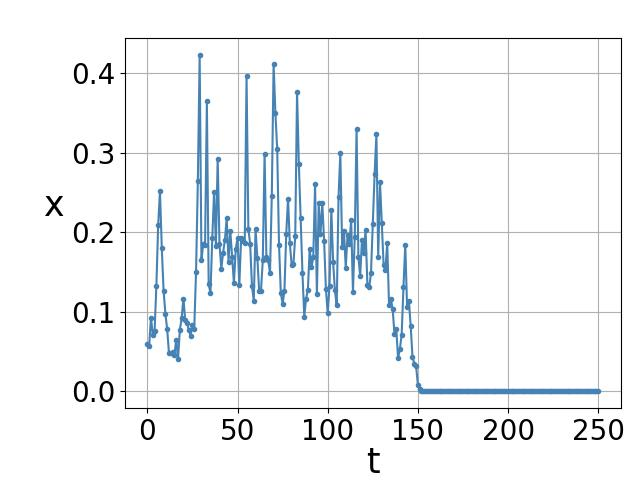
\includegraphics[width=0.5\textwidth]{stochastic/images/time_series_x_0_06_a_1_b_0_56_beta_chaos_epsilon_0_04_fall.jpg}
            \label{time_series_x_0_06_a_1_b_0_56_beta_chaos_epsilon_0_04_fall}
        }
        \subfloat[Выживание]{
            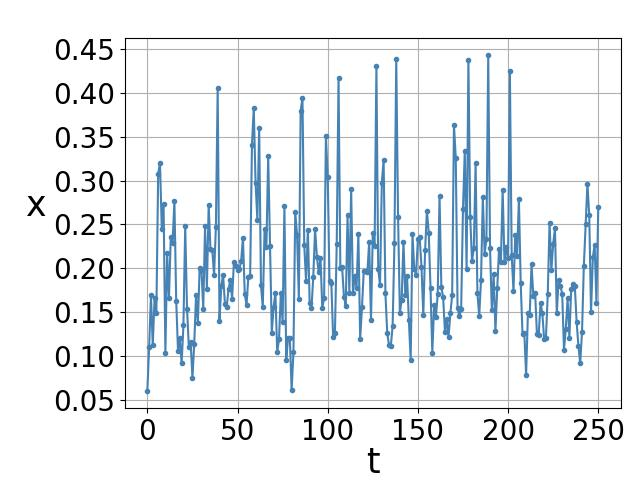
\includegraphics[width=0.5\textwidth]{stochastic/images/time_series_x_0_06_a_1_b_0_56_beta_chaos_epsilon_0_04_alive.jpg}
            \label{time_series_x_0_06_a_1_b_0_56_beta_chaos_epsilon_0_04_alive}
        }  
        
        \captionsetup{justification=centering}
        \caption{Временные ряды модели (\ref{beta_chaos}) при \(\beta = 0.56, \alpha = 1, x_0 = 0.06, \varepsilon = 0.04\)}
    \end{figure}


    % \begin{figure}
    %     \centering
    %     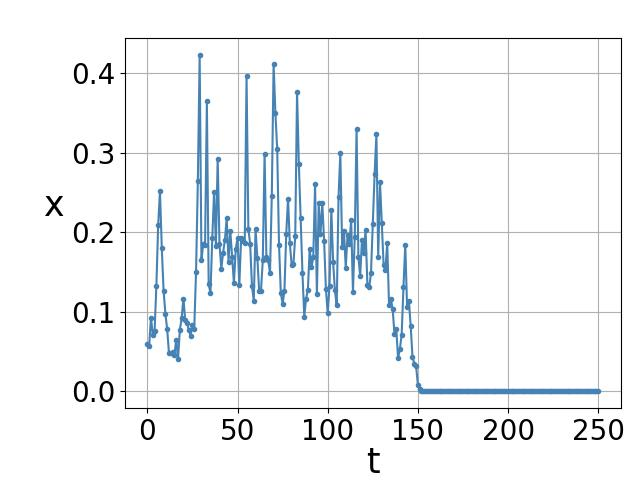
\includegraphics[width=\textwidth]{stochastic/images/time_series_x_0_06_a_1_b_0_56_beta_chaos_epsilon_0_04_fall.jpg}
        
    %     \captionsetup{justification=centering}
    %     \caption{Временной ряд модели (\ref{beta_chaos}) при \(\beta = 0.56, \alpha = 1, x_0 = 0.06, \varepsilon = 0.04\)}
    %     \label{time_series_x_0_06_a_1_b_0_56_beta_chaos_epsilon_0_04_fall}
    % \end{figure}

    % \begin{figure}
    %     \centering
    %     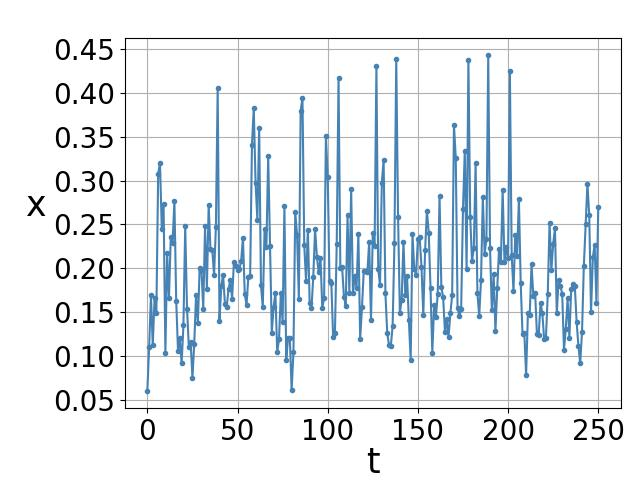
\includegraphics[width=\textwidth]{stochastic/images/time_series_x_0_06_a_1_b_0_56_beta_chaos_epsilon_0_04_alive.jpg}
        
    %     \captionsetup{justification=centering}
    %     \caption{Временной ряд модели (\ref{beta_chaos}) при \(\beta = 0.56, \alpha = 1, x_0 = 0.06, \varepsilon = 0.04\)}
    %     \label{time_series_x_0_06_a_1_b_0_56_beta_chaos_epsilon_0_04_alive}
    % \end{figure}

    При добавлении в модель случайных событий ее поведение становится непредсказуемым. Случайные траектории, под действием шума определенной интенсивности покидают бассейн притяжения детерминированного аттрактора и переходят на вырожденное равновесие \(0\). То есть наблюдается индуцированное шумом вымирание популяции. 
